% Parte 3: o Metodo 1 nas duas tabelas de restricao de fonte do deck
% 2026-10_progresso (sections/03_restricoes_S.tex), como em
% reports/investigating_v2/tabelas.tex (2026-10-09), sem as linhas do Metodo 2.
% Braços anteriores: figures/source_face_3d_vent/SUMMARY.md. Metodo 1:
% problems/screened_poisson/outputs/method1_lu_20k{,_chamber,_lat}.

\section{O Método 1 nos ventrículos (pac2)}

\begin{frame}{O experimento: a verdade das restrições de fonte}
  \small
  \begin{itemize}\setlength{\itemsep}{0.3em}
    \item Ventrículos pac2 (7387 nós); duas fontes endocárdicas, VE e VD, em $t = 0$.
    \item Dois desenhos de $S$: \textbf{chamber} ($S$ = endocárdio do VE; a fonte do VD fica fora de $S$) e \textbf{recoverable} ($S$ = os dois endocárdios).
    \item Método 0: as restrições de fonte do deck anterior; $c$ na verdade $\pm 5\%$, 8 repetições.
    \item Método 1: só ECG, $\varepsilon = 2$ ms, 3 repetições; $c$ na verdade $\pm 30\%$, partindo de $+10\%$. Controle: Método 1 só com LAT.
  \end{itemize}
  \vfill
  {\scriptsize\color{gray} Comparação não controlada: caixa de $c$, passo e penalidades diferem entre os braços.}
\end{frame}

% Teste direto, sem treino: tools/camps_gstar/fit_g_vent.py (.119, 2026-10-16),
% outputs/vent_gstar_{recoverable,chamber}_e2; cv verdadeiro em todo o operador.
\begin{frame}{Antes do inverso: o Método 1 com $g$ dado}
  \footnotesize
  Mesma verdade, $S$ e eletrodos; velocidades verdadeiras, $\varepsilon = 2$ ms.
  $g_0 = \tau^*$ em $S$; $g^*$ = $g$ em $S$ que minimiza o erro de LAT, partindo de $g_0$.\par
  \medskip
  \centering
  \scriptsize
  \setlength{\tabcolsep}{5pt}
  \begin{tabular}{@{}llccccccc@{}}
    \toprule
    desenho & & \shortstack{LAT MAE\\(ms)} & \shortstack{LAT rms\\(ms)} & corr & eik & basins & \shortstack{dispersão\\nas fontes (ms)} & ECG\\
    \midrule
    & verdade & -- & -- & -- & 0,231 & 2 & 0,00 & --\\
    \midrule
    recoverable & $g_0 = \tau^*$ em $S$ & 1,311 & 1,583 & 0,9672 & 0,222 & 2 & 1,72 & 0,299\\
    \tiny ($S$: 3201 nós) & $g^*$ (ajuste ao LAT) & 0,216 & 0,285 & 0,9980 & 0,222 & 3 & 0,58 & 0,032\\
    \midrule
    chamber & $g_0 = \tau^*$ em $S$ & 5,161 & 6,152 & 0,4224 & 0,197 & 1 & 20,02 & 1,282\\
    \tiny ($S$: 1542 nós) & $g^*$ (ajuste ao LAT) & 3,586 & 4,648 & 0,5279 & 0,208 & 4 & 12,04 & 1,638\\
    \bottomrule
  \end{tabular}\par
  \medskip
  {\tiny ECG: erro relativo contra o ECG da verdade. dispersão nas fontes: $\max - \min$ de $\varphi$ nos nós das duas fontes verdadeiras.
  Demais colunas como no slab.}
\end{frame}

\begin{frame}{Antes do inverso: mapas com $g$ dado}
  \centering
  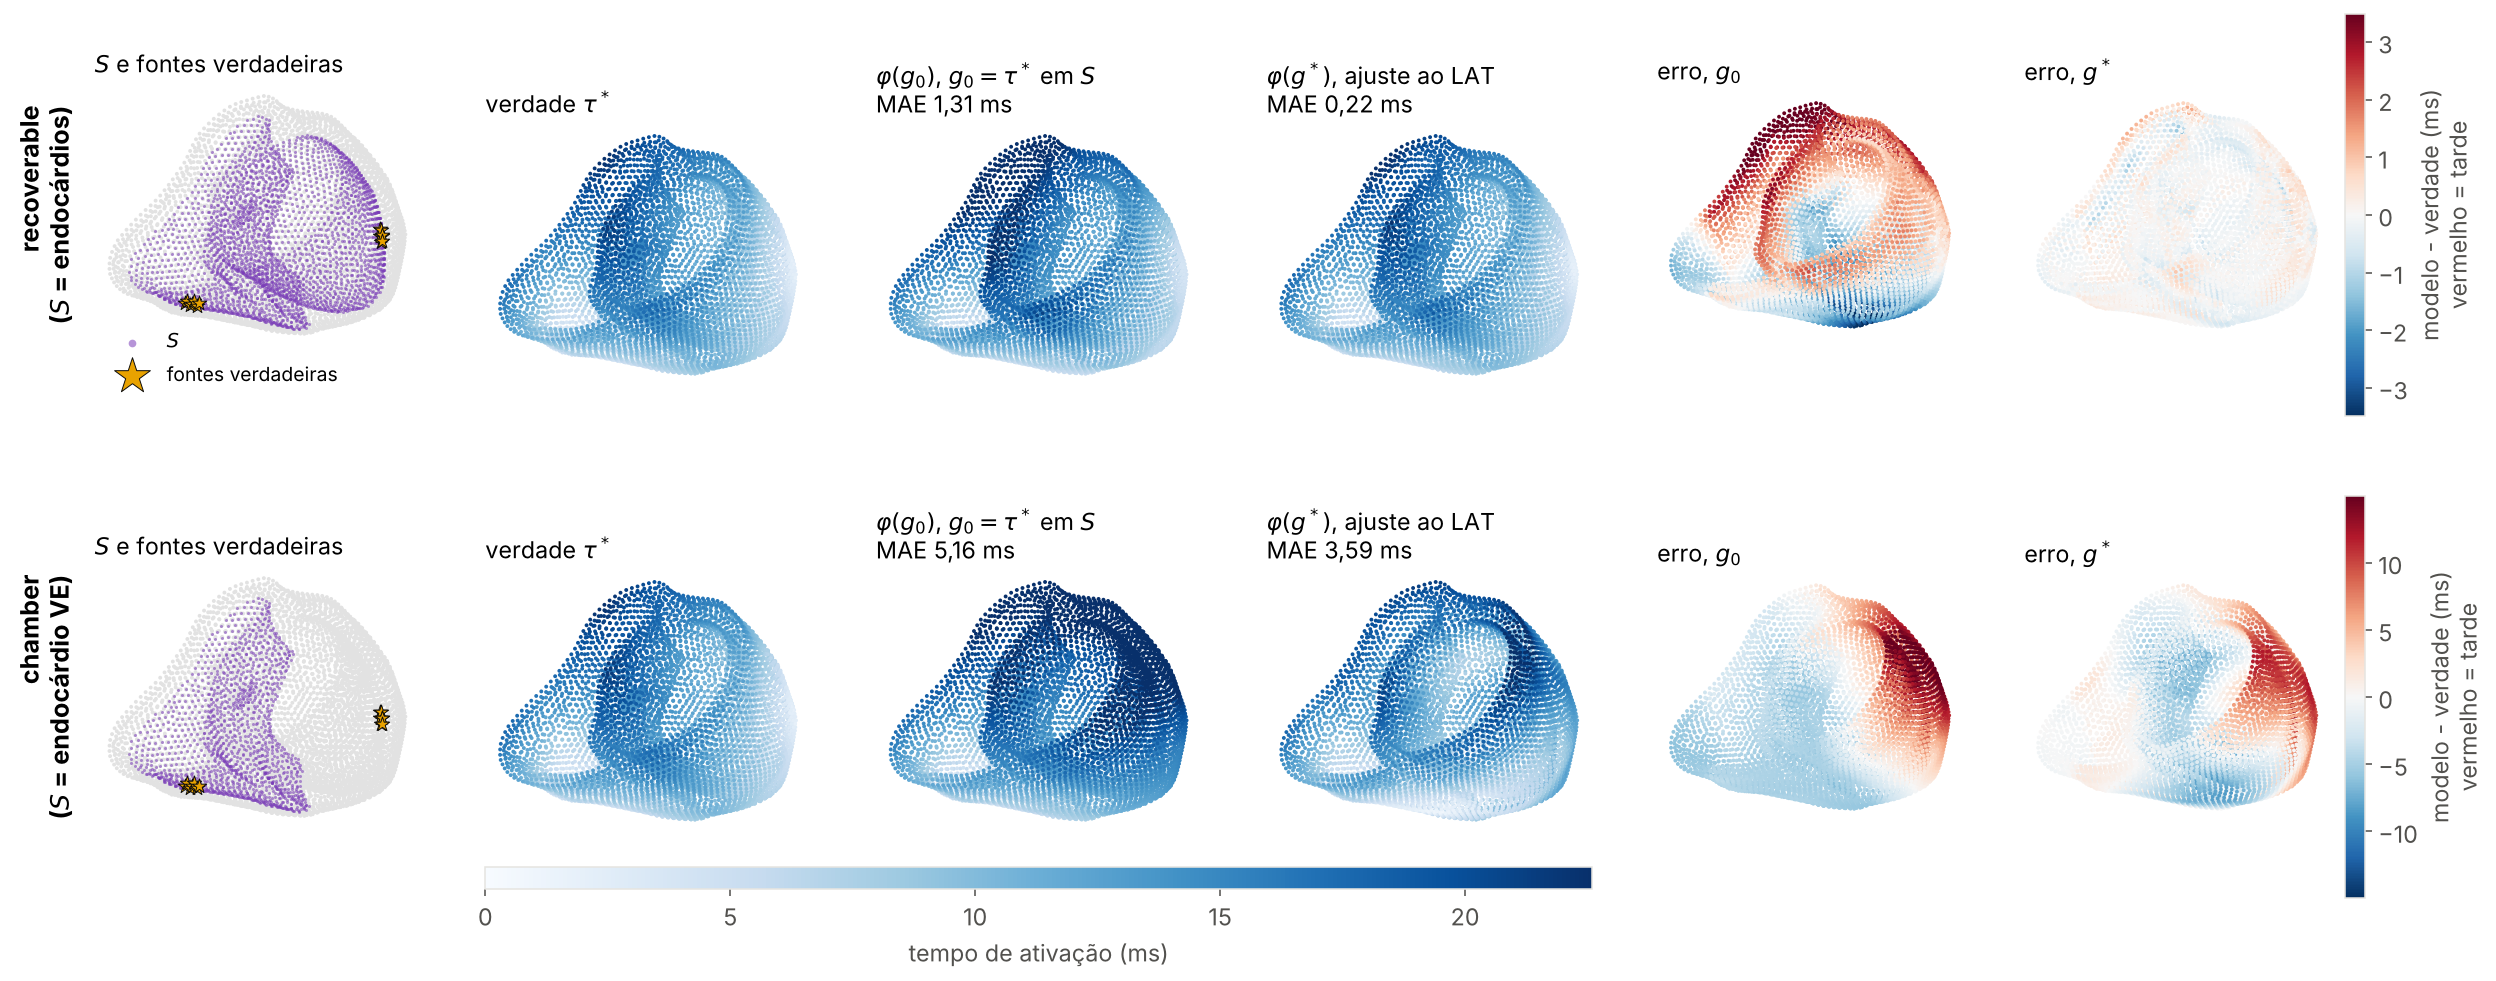
\includegraphics[width=\linewidth]{vent_mapas.png}\par
  {\scriptsize Roxo: $S$; estrelas: as fontes verdadeiras (no chamber, a do VD fica fora de $S$). Erro com as médias removidas.}
\end{frame}

\begin{frame}{Antes do inverso: ECG com $g$ dado}
  \centering
  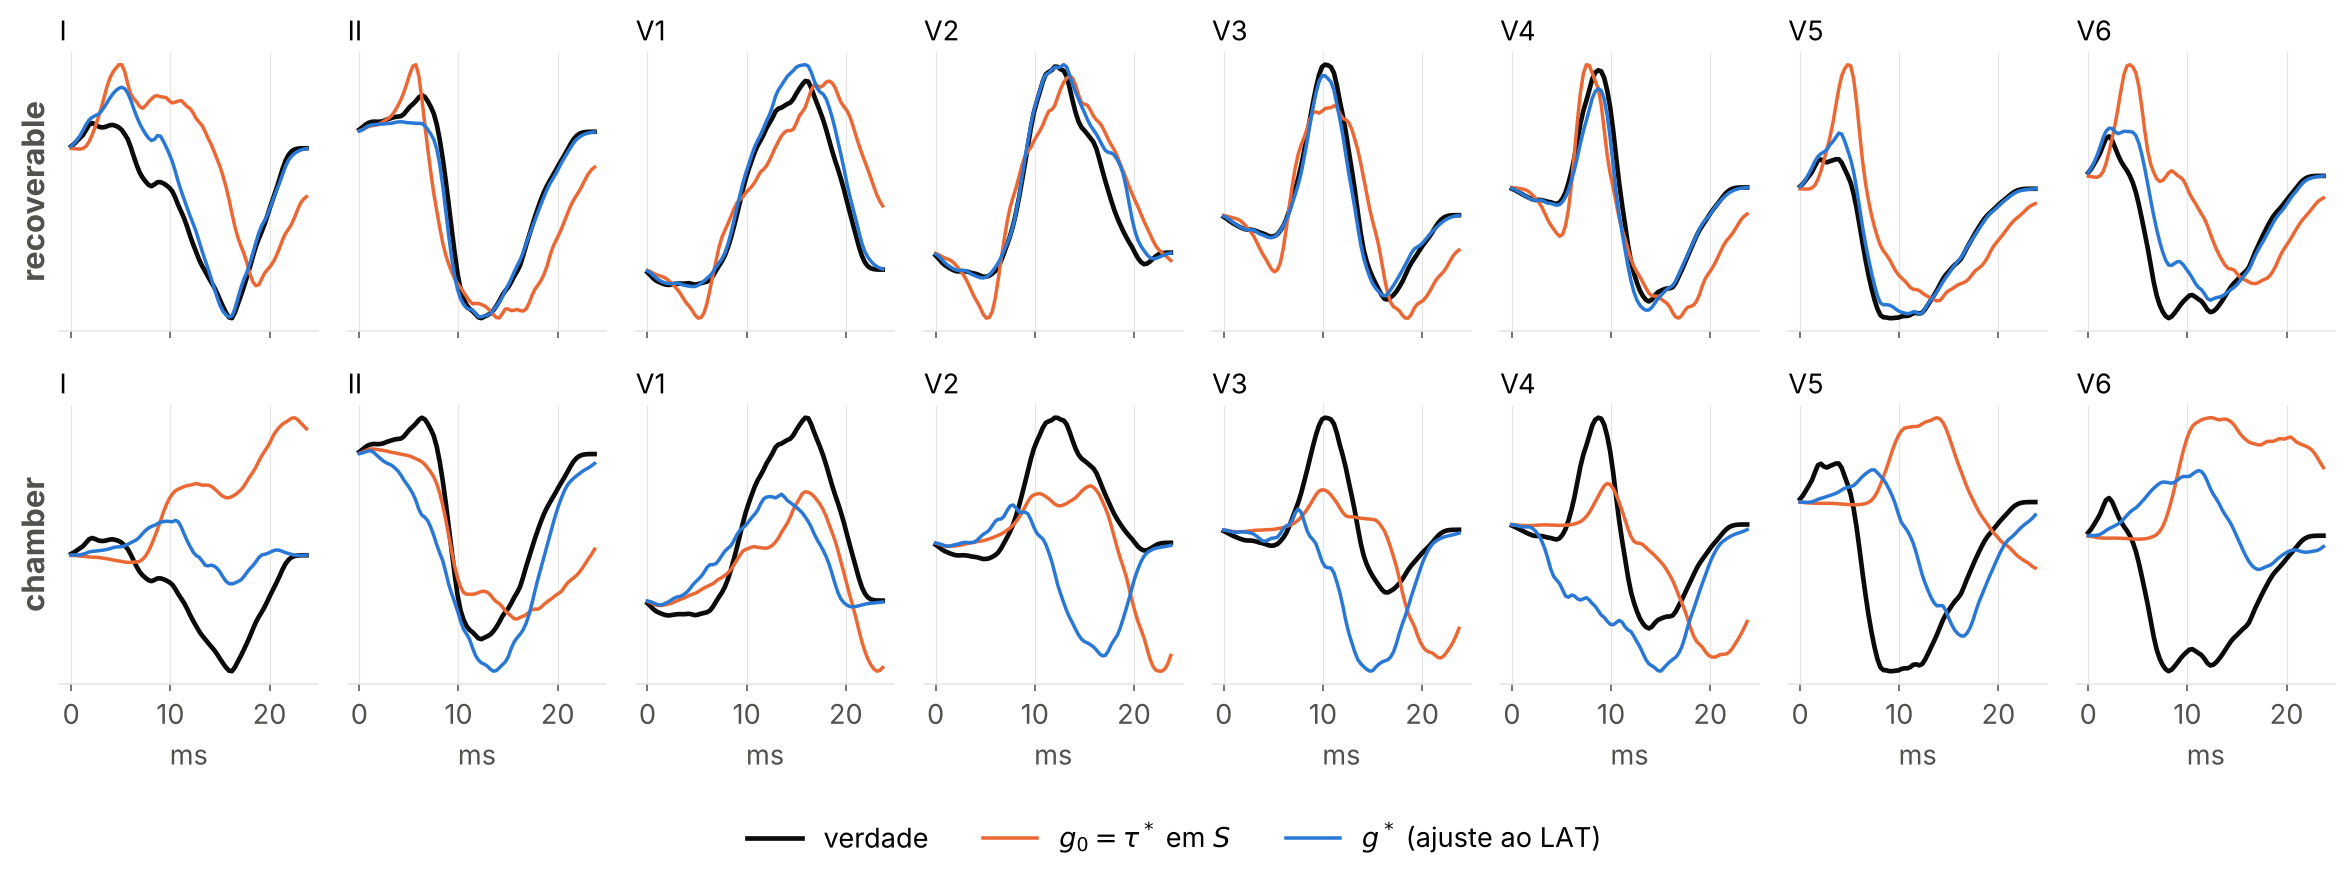
\includegraphics[width=\linewidth]{vent_ecg.png}\par
  {\small Erro relativo do ECG: recoverable $g_0$ 0,299, $g^*$ 0,032; chamber $g_0$ 1,282, $g^*$ 1,638.}
\end{frame}

\begin{frame}[label=tab_camara]{Inverso: chamber ($S$ = endocárdio do VE)}
  \centering
  \scriptsize
  \setlength{\tabcolsep}{5pt}
  \renewcommand{\arraystretch}{0.95}
  \begin{tabular}{@{}lcccccccc@{}}
    \toprule
    braço & ECG & corr & eik & $n$ & \shortstack{prof.\ 2ª\\(ms)} & \shortstack{$d_S$\\fonte 1} & \shortstack{$d_S$\\fonte 2} & \shortstack{$d_S$\\fonte 3}\\
    \midrule
    verdade & -- & -- & 0,231 & 2 & 8,9 & 0,00 & 0,50 & --\\
    sem $L_S$ & 0,010 & 0,57 & 0,172 & 1 & 0,0 & 0,43 {\tiny(8)} & 0,35 {\tiny(3)} & 0,03 {\tiny(2)}\\
    classic, $W=1$ & 0,034 & 0,72 & 0,223 & 2 & 3,5 & 0,01 {\tiny(8)} & 0,38 {\tiny(8)} & 0,00 {\tiny(3)}\\
    ring $k=1$, $W=1$ & 0,014 & 0,56 & 0,191 & 1 & 0,0 & 0,37 {\tiny(8)} & 0,46 {\tiny(3)} & 0,00 {\tiny(1)}\\
    ring $k=1$, $W=100$ & 0,038 & 0,48 & 0,237 & 1 & 0,0 & 0,27 {\tiny(8)} & 0,23 {\tiny(2)} & --\\
    floor, $W=1$ & 0,028 & 0,59 & 0,229 & 3 & 2,1 & 0,02 {\tiny(8)} & 0,40 {\tiny(7)} & 0,09 {\tiny(5)}\\
    floor, $W=100$ & 0,121 & 0,32 & 0,242 & 1 & 0,0 & 0,00 {\tiny(8)} & 0,00 {\tiny(3)} & 0,00 {\tiny(1)}\\
    \midrule
    \textbf{Método 1}, só ECG & 0,173 & 0,28 & 0,436 & 3 & 4,4 & 0,00 {\tiny(3)} & 0,00 {\tiny(3)} & 0,00 {\tiny(3)}\\
    \bottomrule
  \end{tabular}\par
  \medskip
  {\tiny ECG: erro relativo do ECG. corr: correlação com o mapa verdadeiro. eik: RMS de $\|\U\nabla\varphi\| - 1$.
  $n$: fontes com profundidade $\geq 1$ ms; prof.\ 2ª: profundidade da segunda fonte.
  $d_S$ fonte $k$: distância a $S$ da $k$-ésima fonte mais funda (entre parênteses, em quantas repetições ela aparece). Medianas sobre as repetições.}
\end{frame}

\begin{frame}[label=tab_recuperavel]{Inverso: recoverable ($S$ = endocárdios)}
  \centering
  \scriptsize
  \setlength{\tabcolsep}{3.7pt}
  \renewcommand{\arraystretch}{0.86}
  \begin{tabular}{@{}lccccccccc@{}}
    \toprule
    braço & rep. & ECG & corr & eik & $n$ & \shortstack{prof.\ 2ª\\(ms)} & \shortstack{$d_S$\\fonte 1} & \shortstack{$d_S$\\fonte 2} & \shortstack{$d_S$\\fonte 3}\\
    \midrule
    verdade &  & -- & -- & 0,231 & 2 & 8,9 & 0,00 & 0,00 & --\\
    sem $L_S$ & 8 & 0,010 & 0,57 & 0,172 & 1 & 0,0 & 0,00 {\tiny(8)} & 0,00 {\tiny(3)} & 0,03 {\tiny(2)}\\
    classic, $W=1$ & 8 & 0,010 & 0,53 & 0,174 & 1 & 0,0 & 0,00 {\tiny(8)} & 0,07 {\tiny(2)} & 0,00 {\tiny(1)}\\
    ring $k=1$, $W=1$ & 3 & 0,010 & 0,78 & 0,206 & 2 & 3,8 & 0,00 {\tiny(3)} & 0,01 {\tiny(2)} & 0,00 {\tiny(1)}\\
    ring $k=1$, $W=10$ & 3 & 0,016 & 0,53 & 0,220 & 1 & 0,0 & 0,02 {\tiny(3)} & 0,00 {\tiny(1)} & 0,00 {\tiny(1)}\\
    ring $k=1$, $W=100$ & 3 & 0,103 & 0,20 & 0,232 & 1 & 0,0 & 0,05 {\tiny(3)} & -- & --\\
    ring $k=3$, $W=1$ & 3 & 0,010 & 0,52 & 0,171 & 1 & 0,0 & 0,00 {\tiny(3)} & -- & --\\
    ring $k=3$, $W=10$ & 3 & 0,022 & 0,52 & 0,208 & 1 & 0,0 & 0,00 {\tiny(3)} & 0,08 {\tiny(1)} & --\\
    ring $k=3$, $W=100$ & 3 & 0,055 & 0,69 & 0,333 & 2 & 2,7 & 0,04 {\tiny(3)} & 0,00 {\tiny(2)} & 0,00 {\tiny(1)}\\
    ring $k=6$, $W=1$ & 3 & 0,060 & 0,29 & 0,306 & 2 & 1,3 & 0,07 {\tiny(3)} & 0,00 {\tiny(2)} & --\\
    ring $k=6$, $W=10$ & 3 & 0,148 & $-$0,04 & 0,428 & 1 & 0,0 & 0,06 {\tiny(3)} & -- & --\\
    ring $k=6$, $W=100$ & 3 & 0,250 & 0,33 & 0,274 & 1 & 0,0 & 0,06 {\tiny(3)} & -- & --\\
    floor, $W=1$ & 8 & 0,010 & 0,60 & 0,169 & 1 & 0,0 & 0,00 {\tiny(8)} & 0,00 {\tiny(3)} & --\\
    floor, $W=10$ & 8 & 0,013 & 0,52 & 0,165 & 1 & 0,0 & 0,00 {\tiny(8)} & 0,00 {\tiny(1)} & --\\
    floor, $W=100$ & 8 & 0,022 & 0,61 & 0,165 & 1 & 0,0 & 0,00 {\tiny(8)} & 0,00 {\tiny(2)} & --\\
    \midrule
    \textbf{Método 1}, só LAT & 3 & 0,027 & 1,00 & 0,194 & 2 & 8,6 & 0,00 {\tiny(3)} & 0,00 {\tiny(3)} & --\\
    \textbf{Método 1}, só ECG & 3 & 0,002 & 0,81 & 0,236 & 5 & 5,8 & 0,00 {\tiny(3)} & 0,00 {\tiny(3)} & 0,00 {\tiny(3)}\\
    \bottomrule
  \end{tabular}\par
  \medskip
  {\tiny Colunas como na página anterior; rep.: número de repetições.}
\end{frame}
